\documentclass[../notes.tex]{subfiles}

\pagestyle{main}
\renewcommand{\chaptermark}[1]{\markboth{\chaptername\ \thechapter\ (#1)}{}}
\setcounter{chapter}{7}

\begin{document}




\chapter{Molecular Relations \& Quantification}
\section{Machine Learning}
\begin{itemize}
    \item \marginnote{10/22:}Lecture 12 recap.
    \begin{itemize}
        \item Different electronic parameters capture different features of molecules.
        \item Electronic parameters.
        \begin{itemize}
            \item Hammett parameters ($\sigma$).
            \begin{itemize}
                \item Examples include $\sigma_p$, $\sigma_m$, $\sigma^+$, and $\sigma^-$.
            \end{itemize}
            \item Nucleophilicity and electrophilicity.
            \begin{itemize}
                \item Examples include Mayr and Swain-Scott.
            \end{itemize}
            \item NMR or IR shifts.
            \item You can also parameterize via the energy of certain electrons (e.g., $\sigma$, $\sigma^*$, lp, etc.).
        \end{itemize}
        \item Steric parameters.
        \begin{itemize}
            \item A values: Historic.
            \item Sterimol ($L$, $B_1$, and $B_5$): Common.
            \item Taft ($E_s$) and Charton for stereoelectronic.
            \item Bite angle, cone angle, and PBV for sterics in catalysis.
        \end{itemize}
        \item Why do we use parameters?
        \begin{itemize}
            \item Correlating parameters to reaction outcomes (e.g., rate, selectivity, etc.) lets us\dots
            \begin{itemize}
                \item Predict reaction outcomes;
                \item Design better catalysts;
                \item Learn something about the reaction mechanism (this is especially important for this class).
            \end{itemize}
        \end{itemize}
    \end{itemize}
    \item Announcements.
    \begin{itemize}
        \item Don't forget the exam!
        \item This is Masha's last lecture. Fill out the teaching evaluations for Masha and Jonathan at the end of the course! Masha's evals will influence her tenure decision, and Jonathan's could help win him a teaching award.
    \end{itemize}
    \item Today: More complex relationships between the input parameters from last time and our output.
    \begin{itemize}
        \item This is machine learning (ML)!
        \item Masha will focus on the applications of ML to organic chemistry, but please read more about the math and other applications if you're interested!
    \end{itemize}
    \item There will be a lot of vocab in this lecture, starting with the definition of \textbf{AI}.
    \item \textbf{Artificial intelligence}: The development of computer systems able to perform tasks that normally require human intelligence. \emph{Also known as} \textbf{AI}.
    \item Examples of such tasks.
    \begin{itemize}
        \item Speech recognition, decision making, visual perception.
        \item Not just things like calculus, but things that require a "greater" level of intelligence.
    \end{itemize}
    \item Under the umbrella of AI falls \textbf{ML}.
    \item \textbf{Machine learning}: A subfield of AI that allows computer systems to learn and adapt without explicit instructions or programming. \emph{Also known as} \textbf{ML}.
    \begin{itemize}
        \item ML is characterized by the computer system being able to do things that we didn't explicitly program it to do.
    \end{itemize}
    \item In the context of ML, we also have an explicit definition of \textbf{learning}.
    \item \textbf{Learning}: A computer program is said to form some experience ($E$) with respect to a task ($T$) and a measure of performance ($P$; aka the "performance metric"), if it's performance on $T$ --- as measured by $P$ --- improves with $E$.
    \begin{itemize}
        \item This gets into the Turing test, and what it really means to know and to learn and to be conscious. This is more the realm of philosophy, and we won't get into that.
        \item It's not like it did great from the beginning; it's that it had to get better with more experience.
    \end{itemize}
    \item Reviews on the subject of ML in chemistry.
    \begin{itemize}
        \item A great one to start for organic chemists: \textcite{bib:MLChemRev}. Four big-name corresponding authors.
        \begin{itemize}
            \item Tobias Gensch: He's new, but we'll know him soon.
            \item Sigman: The pioneer of multivariate linear regression.
            \item Doyle: First to publish ML in chemistry; her 2018 \emph{Science} paper --- \textcite{bib:DoyleML} --- exploded the field.
            \item Anslyn: Wrote our textbook; the gold standard of Phys Orgo.
        \end{itemize}
        \item Any review publsihed by Doyle or Sigman will be great to read.
        \item There are also great reviews from Connor Coley, Bill Green, and Klavs Jensen.
    \end{itemize}
    \item Types of learning: \textbf{Supervised} and \textbf{unsupervised}.
    \item \textbf{Supervised} (learning): ML that has \textbf{labeled} training data.
    \begin{itemize}
        \item This type of ML analyzes the labeled data and then makes a guess on unlabeled data. After the model guesses, we evaluate its performance.
        \item Example: Show my model 100 reactions (with their yields labeled), and then have it guess the yield of a new reaction it's never seen before.
        \item This is called "supervised" learning, because after the model guesses, \emph{we} need to show it the right answer (i.e., the label).
        \item Example: Spam filters.
        \begin{itemize}
            \item These separate spam from "ham," the technical term for good emails.
            \item We train such models by showing them a bunch of spam emails and a bunch of ham emails so that they "learn" what spam looks like.
            \item The model looks for typos, weird email addresses, requests for money, etc.
        \end{itemize}
    \end{itemize}
    \item \textbf{Labeled} (training data): A set of data in which each data point (or datum) has an input and output label.
    \item \textbf{Unsupervised} (learning): ML that has \textbf{unlabeled} training data.
    \begin{itemize}
        \item This type of ML tries to uncover relationships between data and find patterns.
        \item This is "unsupervised" because there is no right answer, no guidance, no yield.
        \item A common approach: \textbf{Clustering}.
        \item Example: Netflix recommends movies that are similar to each other (i.e., which share common actors, common runtime, common genre labels, common people who have watched them, etc.).
    \end{itemize}
    \item \textbf{Clustering}: Grouping together similar data.
    \item A really common approach is to do both of these at once in \textbf{semi-supervised} learning, our secret third option.
    \item \textbf{Semi-supervised} (learning): ML that splits data into a small labeled dataset and a big unlabeled dataset.
    \begin{itemize}
        \item We group data together and assign a label to the group.
        \item Example: Image classification, i.e., to answer the question, "which photos are of the same animal?"
        \begin{itemize}
            \item An unsupervised ML finds similar images, and then a few of those get labeled "cat," so the whole group gets labeled "cat."
            \item This is how self-driving cars and Captcha work. When you help Captcha find all the images with stairs, you're (nonconsensually) providing labels to help train image recognition models!
        \end{itemize}
    \end{itemize}
    \item We'll focus on supervised learning for the rest of today.
    \item Two types of supervised learning: \textbf{Classification} and \textbf{regression}.
    \item \textbf{Classification}: The output/label is a category.
    \begin{itemize}
        \item There are a finite number of options.
        \item Example: Photos are "cat," "dog," or "human."
    \end{itemize}
    \item \textbf{Regression}: The output/label is a continuous number.
    \begin{itemize}
        \item There are an infinite number of options.
        \item Example: We could model the cost of a house as a function of house properties (e.g., the year it was built, the year we're trying to buy it, the cost of the surrounding homes, the neighborhood school system, etc.).
        \item Example: Model $\Delta G$ as a function of reaction parameters.
        \begin{itemize}
            \item This is Hammett plots! That was linear regression, so that's why we call this, "regression."\footnote{Is there a "second time you hear it" effect in psychology that mimics ML? Unlikely to place emphasis on something the first time we hear it (e.g., Dad saying that there are crazy jobs for smart people/Maya telling me about the email tracker), but more likely when we hear it again (e.g., Carina Hong's job/Dylan Miars telling me about the email tracker). Relation to retention in learning!}
        \end{itemize}
        \item Far more common in chemistry.
        \item Formal definition: A statistical technique for determining the relationship between independent or explanatory variables ($x$) and dependent or response variables ($y$).
    \end{itemize}
    \item \textbf{Linear regression}: Describe the relationship between $x$ and $y$ as a straight line.
    \begin{itemize}
        \item Fitting to $y=mx+b$.
        \item Example: $\log(k_{\ce{X}}/k_{\ce{H}})=\rho\sigma$.
        \item Some people don't call this ML; they call this "statistics." But that distinction is really only fought over by people who care about semantics or credit. So you may hear some strong opinions in the field (e.g., Sigman doesn't call it ML), but it's just labels at the end of the day (in Masha's opinion).
    \end{itemize}
    \item \textbf{Multivariate} (linear regression): Multiple $x$ and $y$ variables.
    \begin{itemize}
        \item This is all the work of Matt Sigman, building off of his classic Hammett paper (Figure \ref{fig:multiLFER}) that we reviewed last lecture.
    \end{itemize}
    \item The ML workflow: Here are the steps if you want to go into lab and plan a project.
    \begin{enumerate}[start=0]
        \item Know or define your goal and application.
        \begin{itemize}
            \item Why do you want this model?
            \item What do you want it to do?
            \item Why do you want to use it?
            \item Why would anyone care about it?
            \item A model that can predict yield to a decimal point will need tens of thousands of data points.
            \begin{itemize}
                \item If you want a model to help you refine a ligand for a reaction that you've already studied pretty well, that's a good use.
            \end{itemize}
            \item ML is fundamentally an engineering solution, so you better have a practical use for this tool you've built.
        \end{itemize}
        \item Data collection.
        \begin{itemize}
            \item How much data?
            \item Labeled or unlabeled?
            \item Will this data come from the literature or from experiment?
            \begin{itemize}
                \item This is an especially relevant consideration in chemistry.
            \end{itemize}
            \item Be aware of bias; we, as a field, tend to overreport high-yield reactions and underreport low-yield reactions. So if we train a model based just on the literature, it will think all chemical reactions are high yield.
            \item The adage here: Garbage in = garbage out.
            \begin{itemize}
                \item If you train a model on bad data, you're going to have a bad model.
            \end{itemize}
            \item So we can go into the lab and get a bunch of low-yield reactions and feel good about it, which almost never happens!
            \item Warning: If you go to Reaxys and dump a bunch of data into a model, the error rate is 30-60\% (typos and such).
            \begin{itemize}
                \item Notoriously, the patent database used to be 60\% wrong due to bad data-scraping.
            \end{itemize}
        \end{itemize}
        \item \textbf{Parameterization}.
        \begin{itemize}
            \item Categorical descriptors (common for solvents, salts, and additives).
            \begin{itemize}
                \item Tell your model that these 10 were run in toluene, these 10 in DCM, etc. That's a common category approach.
            \end{itemize}
            \item Chemically meaningful parameters.
            \begin{itemize}
                \item This is all of last lecture: $\sigma$ values, sterimol values, etc.
                \item These are chemically meaningful because they capture a feature important to reactivity.
            \end{itemize}
            \item Graph networks: Atoms are nodes, bonds are edges, etc.
            \item Molecular fingerprints: Lists of functional groups.
            \begin{itemize}
                \item Example: My molecule contains a ketone, an ester, two methynes, etc.
            \end{itemize}
            \item SMILES, or its derivatives: This is how ChemDraw encodes molecules.
            \begin{itemize}
                \item Example: Cyclohexane is "C1CCCCC1".
                \item This string is just text, so then we can use LLMs.
                \item Masha doesn't think these work that well, but they do exist.
            \end{itemize}
            \item Most ML papers mess up by this point: They either got bad data, or misrepresented it.
            \item Most ML applications use millions or billions of datapoints, so chemistry is a bit unique in that it uses dozens of data points. How to make that tenable is a big question in both the chemistry and computer science communities!
        \end{itemize}
        \item Data preprocessing: Cleaning up the data for modeling.
        \begin{itemize}
            \item Technique: Normalization.
            \begin{itemize}
                \item Make all parameters lie in the range of 0-1.
                \begin{itemize}
                    \item To do this, just divide by the maximum value.
                \end{itemize}
                \item Example: Sterimol values of 1, 4, and 8 become 0.125, 0.5, and 1; charge values of 0.01, 0.04, and 0.08 become 0.125, 0.5, and 1.
                \item Normalization helps us make sure that the model doesn't think sterimol values are 100 times more important than charge. Essentially, it prevents bias toward parameters with large values.
            \end{itemize}
            \item Technique: Reduce the number of parameters (if needed).
            \begin{itemize}
                \item Sigman recommends 8 data points per single parameter.
                \item If we have more parameters than data points, we have an \textbf{overfit} model (see Figure \ref{fig:MLfitc}), and that is no good.
            \end{itemize}
            \item The simplest model architecture (Occam's razor) is the best model.
        \end{itemize}
        \item Data sampling: Splitting data into \textbf{training}, \textbf{validation}, and \textbf{test} sets.
        \begin{itemize}
            \item We also sometimes have an \textbf{out-of-sample} set.
            \item So we have a model, but just like in science, we need the model to make useful predictions for it to be a good model.
            \item In the validation set, the model is going to show us it's performance.
            \begin{itemize}
                \item Example: If linear regression does 70\% right and multivariate linear regression does 90\% right, we go with the multivariate architecture.
            \end{itemize}
            \item Then the performance of the model that we report is the performance on the final (test) set.
            \item Overexposing your model to the test set invalidates the model; this is called \textbf{data leakage}.
            \item Note: Chemists tend to mix up the "validation" and "test" sets in their writing.
            \begin{itemize}
                \item Just make sure that we have real evidence that the model works on \emph{unseen} data.
                \item If you see people say, "we used the validation set to test the model, and then applied the model to the test set," that's not a bad thing; that's just a semantic error.
            \end{itemize}
        \end{itemize}
        \item Training and testing: Evaluate the performance of different model architectures based on \textbf{metrics}.
        \begin{itemize}
            \item Example metrics: Accuracy, percent data explained, $R^2$, RMSE (root-mean-square error).
            \item Here, we run control and baseline models to predict the average and mode.
        \end{itemize}
        \item Interpretation and prediction: Use the trained model to predict reaction results, guide catalyst design, or present mechanistic hypotheses.
        \begin{itemize}
            \item Best practice: Test the model experimentally.
            \item Relating back to Point 0: Make sure the model is worth making.
            \begin{itemize}
                \item Make sure you use it for something cool; you don't need a chainsaw to hammer in a nail.
            \end{itemize}
        \end{itemize}
    \end{enumerate}
    \item \textbf{Parameterization}: Converting chemical information to \textbf{machine-readable} formats.
    \item \textbf{Machine-readable} (input): A number, binary value, graph representation, etc.
    \item \textbf{Training} (set): The set on which the model learns the trends.
    \begin{itemize}
        \item Roughly 70\% of the data.
    \end{itemize}
    \item \textbf{Validation} (set): The subset of the training set that help you choose between model architectures.
    \item \textbf{Test} (set): The set on which we evaluate the model performance.
    \begin{itemize}
        \item Roughly 30\% of the data.
        \begin{itemize}
            \item The actual numbers here are up to you! People do everything from $90:10$ to $60:40$.
        \end{itemize}
        \item We really only want to use the test set once or twice.
    \end{itemize}
    \item \textbf{Out-of-sample} (set): A set that helps us further validate generalizability or \textbf{extrapolation}. \emph{Also known as} \textbf{experimental validation} (set).
    \item \textbf{Data leakage}: The mixing of data between the test set and the training set. \emph{Also known as} \textbf{poor data hygeine}.
    \item \textbf{Extrapolation}: The ability to make predictions beyond the training set.
    \item Memo: Extrapolation vs. \textbf{interpolation}?
    \begin{itemize}
        \item There definitely is a difference.
        \item For an example of true extrapolation, see Sigman's paper on extrapolating a model trained on ligands with ee below 80\% to find ligands with ee beyond 80\%.
    \end{itemize}
    \item Don't report your training set performance!
    \item \textbf{Overfit} (model): A model that can predict the training set, but not new data.
    \begin{itemize}
        \item Such models cannot generalize, and they definitely cannot extrapolate.
        \item See Figure \ref{fig:MLfitc}.
    \end{itemize}
    \item There are actually three types of fitting.
    \begin{figure}[h!]
        \centering
        \begin{subfigure}[b]{0.3\linewidth}
            \centering
            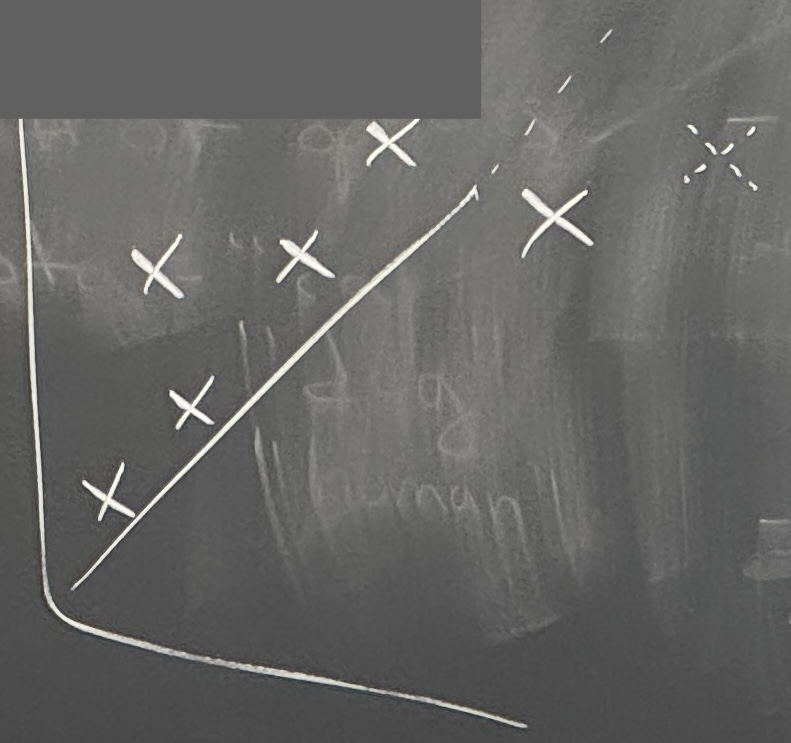
\includegraphics[width=0.63\linewidth]{MLfita.JPG}
            \caption{Underfit.}
            \label{fig:MLfita}
        \end{subfigure}
        \begin{subfigure}[b]{0.3\linewidth}
            \centering
            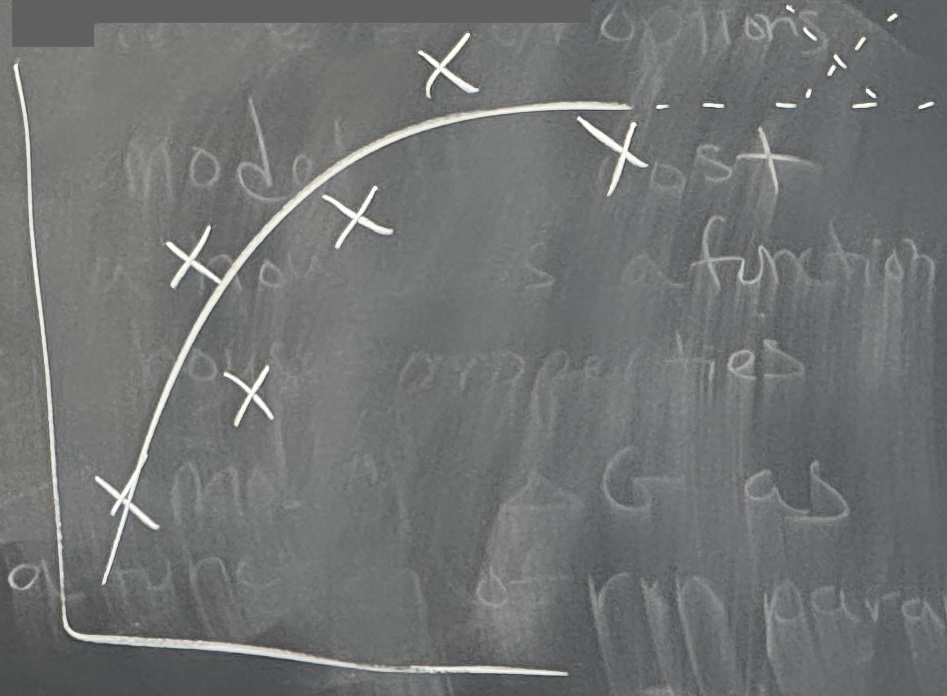
\includegraphics[width=0.8\linewidth]{MLfitb.JPG}
            \caption{Good fit.}
            \label{fig:MLfitb}
        \end{subfigure}
        \begin{subfigure}[b]{0.3\linewidth}
            \centering
            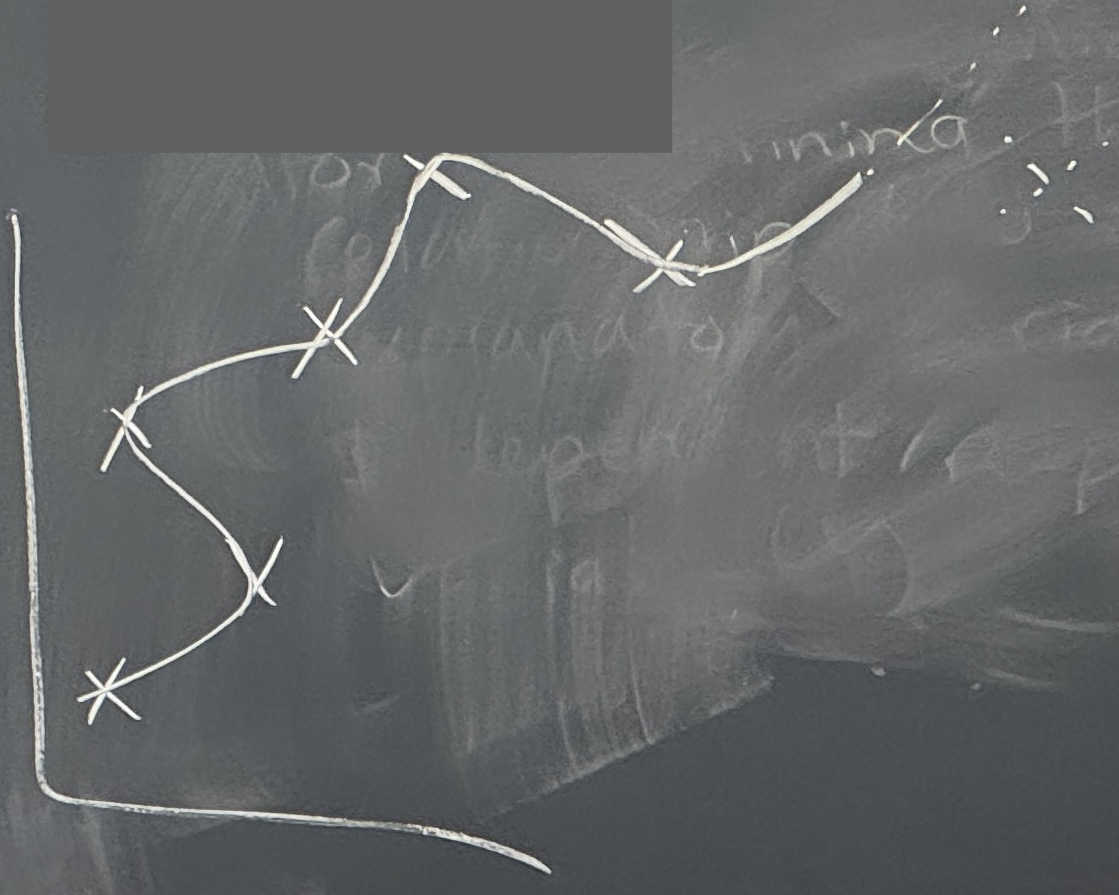
\includegraphics[width=0.74\linewidth]{MLfitc.JPG}
            \caption{Overfit.}
            \label{fig:MLfitc}
        \end{subfigure}
        \caption{Fitting machine learning models.}
        \label{fig:MLfit}
    \end{figure}
    \begin{itemize}
        \item Figure \ref{fig:MLfita}: Underfitting.
        \begin{itemize}
            \item Doesn't generalize to new data.
        \end{itemize}
        \item Figure \ref{fig:MLfitb}: Good fitting.
        \begin{itemize}
            \item Generalizes well to new data.
        \end{itemize}
        \item Figure \ref{fig:MLfitc}: Overfitting.
        \begin{itemize}
            \item Doesn't generalize at all to new data.
            \item This is tempting to chemists, because it gives them a good-looking model. But that's not actual model; that's fraud!
        \end{itemize}
    \end{itemize}
    \item Model architectures.
    \begin{figure}[h!]
        \centering
        \begin{subfigure}[b]{0.2\linewidth}
            \centering
            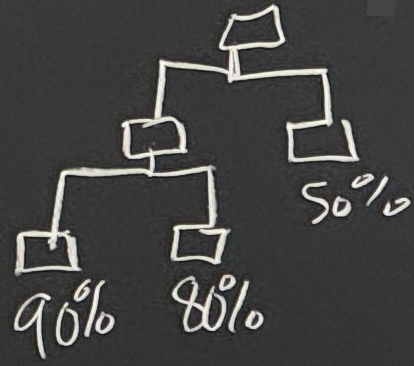
\includegraphics[width=0.8\linewidth]{MLarcha.JPG}
            \caption{Decision tree.}
            \label{fig:MLarcha}
        \end{subfigure}
        \begin{subfigure}[b]{0.2\linewidth}
            \centering
            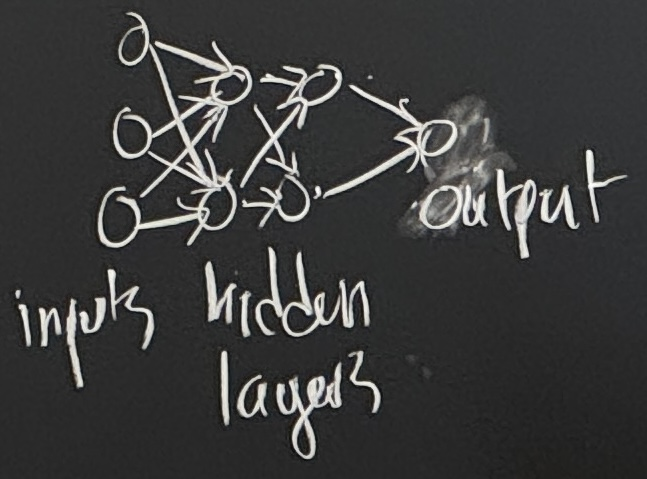
\includegraphics[width=0.9\linewidth]{MLarchb.JPG}
            \caption{Neural network.}
            \label{fig:MLarchb}
        \end{subfigure}
        \caption{Machine learning model architectures.}
        \label{fig:MLarch}
    \end{figure}
    \begin{itemize}
        \item These exist on a spectrum from models with low complexity and high interpretability to models with high complexity and low interpretability.
        \item Lowest complexity and highest interpretability: Linear regression.
        \item $k$-nearest neighbors (knn).
        \begin{itemize}
            \item Basic idea: Our ligand is close to something with high ee, so we'll probably get high ee, too.
        \end{itemize}
        \item Decision trees (Figure \ref{fig:MLarcha}).
        \begin{itemize}
            \item Answer questions such as, "high electronegativity or low electronegativity," and correlates that to ees.
        \end{itemize}
        \item Random forest.
        \begin{itemize}
            \item A subset of decision trees.
            \item Make a lot of trees and average the result.
            \item Called a "forest" because there are many trees!
        \end{itemize}
        \item Highest complexity and lowest interpretability: Neural networks (Figure \ref{fig:MLarchb}).
        \begin{itemize}
            \item Like the brain: Inputs, through hidden layers, that converge on an output.
            \item This year's physics Nobel Prize went to neural networks; Masha's not quite sure how these are physics, but they really have changed their game.
            \item They're very powerful, but extremely complex (so often overfit and not very interpretable).
            \begin{itemize}
                \item Called "black box models."
                \item Not good for mechanisms!
            \end{itemize}
        \end{itemize}
    \end{itemize}
    \item Masha also has some additional notes on model architectures that she will post on Canvas.
\end{itemize}



\section{Noncovalent Interactions}
\begin{itemize}
    \item \marginnote{10/24:}Logistics.
    \begin{itemize}
        \item Alex has led this class for several years at this point, and it is his favorite one to teach!
        \item Goal for the remainder of the semester: Build out an increasingly deep foundation on molecular reactivity.
        \item Thus far, we've learned about the intrinsic reactivity of certain things (e.g., carbenes); from now on, though, Alex will expand beyond intrinsic properties to talk about how molecules behave not only in isolation, but with other molecules and how these bits of reactivity manifest (sometimes in statistical ways).
        \item A lot of stuff going forward may be review from physical chemistry, advanced organic, etc. This is not a problem! That's a feature of the graduate curriculum.
        \begin{itemize}
            \item Especially if you've seen it before, be more inquisitive this time! Once you're familiar, be incisive.
            \item If it's new, that's why we're here! Learn it now.
        \end{itemize}
        \item This should be an interactive lecture: Alex will pose questions and call on people if answers are not forthcoming.
        \item The class style will be chalk-talk. The majority of what we need to know goes on the board, but not all!
        \begin{itemize}
            \item If he riffs and says something exciting, write it down! It will not be in the notes, though.
        \end{itemize}
        \item 2 PSets and 1 exam this half-semester as well.
        \item Exam 1 will likely be returned before next Tuesday.
        \item Class begins at 10:35 on the dot, and Alex will talk until (not past) noon if he has enough to say.
    \end{itemize}
    \item Alex is quite funny!
    \item We've learned a bit thus far about how molecules adopt their equilibrium shape (e.g., with Walsh diagrams).
    \begin{itemize}
        \item Electronic control elements define intrinsic properties, which can tell us a great deal about reactivity.
        \item Frontier MOs are very important, "as Ken Fukui and Roald Hoffmann taught us."
        \item We will now layer on top additional forces that give us greater insight into how molecules behave when in proximity to others.
        \item Unless you're a microwave spectroscopist, most of the chemistry we're interested in happens in a condensed medium.
    \end{itemize}
    \item Later on: How these interactions affect a system, and how stimuli can modify that system.
    \item At the end of the class: Photochemistry and electron transfer, if we move apace.
    \item Today: \textbf{Noncovalent interactions}.
    \begin{itemize}
        \item We'll list a bunch of forces; a not super fun lecture. But we'll reference all these forces going forward.
    \end{itemize}
    \item \textbf{Noncovalent interaction}: An interaction between atoms (stabilizing or destabilizing) that does not occur pairwise through a covalent bond. \emph{Also known as} \textbf{NCI}.
    \begin{itemize}
        \item These are enthalpic and entropic forces that modulate molecular interactions.
    \end{itemize}
    \item \textbf{Electrostatic} (interaction): A charge-charge interaction. \emph{Also known as} \textbf{ion-ion interaction}.
    \begin{itemize}
        \item Even in organic chemistry, a lot of charge densities can be generated.
        \item Example: Ammonium ion held near a carboxylate.
        \item To learn something about the overall energy of a system subject to this interaction, use \textbf{Coulomb's law}.
    \end{itemize}
    \item \textbf{Coulomb's law}: If a charge $q_1$ is held a distance $r$ from a charge $q_2$, the energy of the system is given as follows. \emph{Given by}
    \begin{equation*}
        E = \frac{q_1q_2}{4\pi\epsilon r}
    \end{equation*}
    \emph{Schematic}
    \begin{figure}[h!]
        \centering
        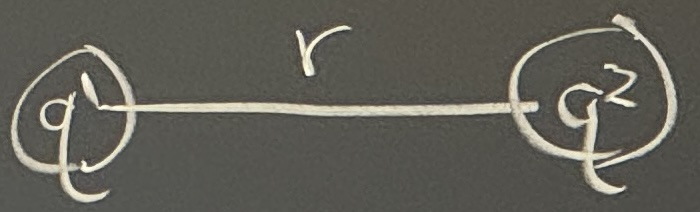
\includegraphics[width=0.2\linewidth]{intElectro.JPG}
        \caption{Schematic of an electrostatic interaction.}
        \label{fig:intElectro}
    \end{figure}
    \begin{itemize}
        \item $\epsilon$ is the \textbf{dielectric constant}.
        \item What's important here is that $\Delta E\propto 1/r$.
        \begin{itemize}
            \item Not all forces have this energy relationship!
        \end{itemize}
    \end{itemize}
    \item \textbf{Dielectric constant}: The ability of a medium to isolate two static charges from each other. \emph{Denoted by} $\bm{\epsilon}$.
    \begin{itemize}
        \item This is \emph{distinct} from $\epsilon_0$, which is the ability of a \emph{vacuum} to isolate two static charges from each other!
        \item \textcite{bib:Anslyn} refers to the permittivity of the medium as $\epsilon_\mu$, and uses $\epsilon$ to denote $\epsilon_\mu/\epsilon_0$.
    \end{itemize}
    \item Example of electrostatic interactions.
    \begin{figure}[H]
        \centering
        \footnotesize
        \begin{subfigure}[b]{\linewidth}
            \centering
            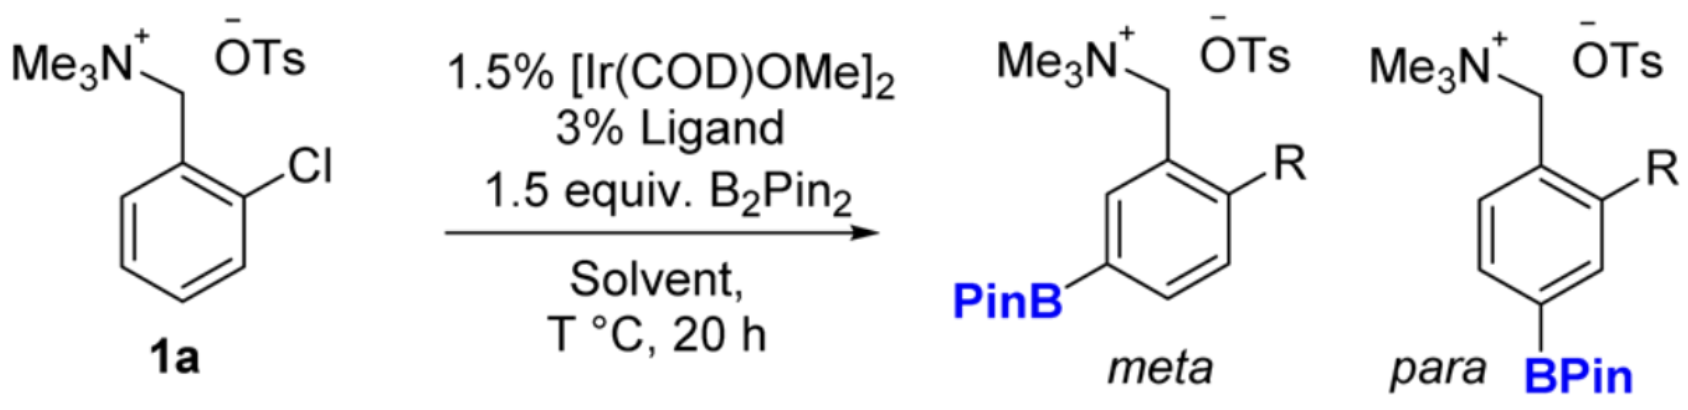
\includegraphics[width=0.6\linewidth]{intElectroLiga.png}
            \caption{Reaction.}
            \label{fig:intElectroLiga}
        \end{subfigure}\\[2em]
        \begin{subfigure}[b]{0.4\linewidth}
            \centering
            \chemfig{*6([:-30]=-N=(-*6(=N-=-(-{}^{\emph{t}}Bu)=-))-=(-{}^{\emph{t}}Bu@{})-)}
            \caption{A bulky ligand (dtbpy).}
            \label{fig:intElectroLigb}
        \end{subfigure}
        \begin{subfigure}[b]{0.4\linewidth}
            \centering
            \chemfig{\phantom{O_3@{}S}-[:-60,,,,opacity=0]-*6(=-N=(-*6(=N-=(--[:60]S@{}\charge{45=$\ominus$}{O}_3)-=-))-=-)}
            \caption{A charged ligand.}
            \label{fig:intElectroLigc}
        \end{subfigure}
        \caption{Electrostatic interactions in catalysis.}
        \label{fig:intElectroLig}
    \end{figure}
    \begin{itemize}
        \item A chloroarene bearing a pendant ammonium ion is subjected to catalytic borylation conditions (Figure \ref{fig:intElectroLiga}).
        \item When a particular ligand is employed (Figure \ref{fig:intElectroLigb}), the catalyst delivers the Bpin to the position remote from the charged group (\emph{para}) favorably over the \emph{meta}-position in a $2:1$ ratio.
        \item However, use of a complementarily charged ligand (Figure \ref{fig:intElectroLigc}) led to the complete inverse regiochemistry --- and with an improved selectivity of $10:1$!
        \item The dielectric can also modify this: More polar solvents with higher dielectrics erode selectivity.
        \item Reference: \textcite{bib:intElectroLig}.
        \begin{itemize}
            \item Also out of the Phipps lab at Cambridge!
        \end{itemize}
    \end{itemize}
    \item \textbf{Charge-dipole} (interaction): An NCI between a point charge and a dipole. \emph{Given by}
    \begin{equation*}
        E = \frac{\mu q_2\cos(\theta)}{4\pi\epsilon r^2}
    \end{equation*}
    \emph{Schematic}
    \begin{figure}[h!]
        \centering
        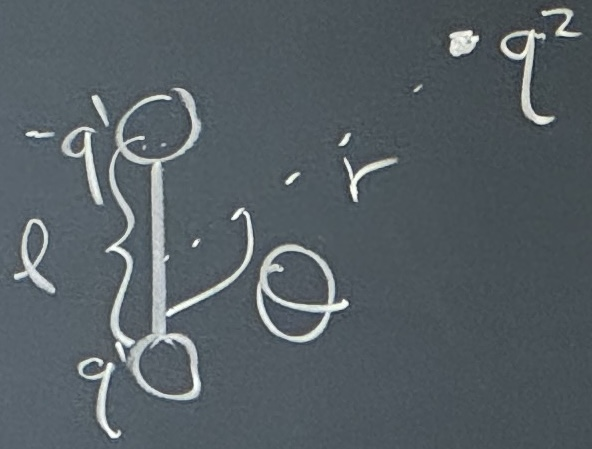
\includegraphics[width=0.15\linewidth]{intCrgDpl.JPG}
        \caption{Schematic of a charge-dipole interaction.}
        \label{fig:intCrgDpl}
    \end{figure}
    \begin{itemize}
        \item $\mu$ is the \textbf{dipole moment}.
        \item We can number charges $q$ with subscripts or superscripts.
        \item Again, higher dielectrics screen the charge better.
        \item Here, $\Delta E\propto 1/r^2$.
        \item Example: The attraction between a carbonyl and a \ce{Li+} ion, e.g., carbonyl activation by a Lewis acid!
    \end{itemize}
    \item \textbf{Dipole moment}: A measure of the separation of positive and negative electrical charges within a system; that is, a measure of the system's overall polarity. \emph{Denoted by} $\bm{\mu}$. \emph{Units} \si{\debye} "debye"
    \item These are both great, but many organic molecules are uncharged.
    \item \textbf{van der Waals} (interaction): An NCI between uncharged molecules.
    \begin{itemize}
        \item Can be either attractive \emph{or} repulsive.
        \item Several subsets.
        \begin{enumerate}[label={\Roman*.)}]
            \item \textbf{Dipole-dipole interactions}.
            \item \textbf{Dipole-induced dipole interactions}.
            \item \textbf{Dispersion forces}.
        \end{enumerate}
    \end{itemize}
    \item \textbf{Dipole-dipole} (interaction): An NCI between two dipoles fixed in the same plane and parallel. \emph{Given by}
    \begin{equation*}
        E = -\frac{\mu_1\mu_2(3\cos^2\theta-1)}{4\pi\epsilon r^3}
    \end{equation*}
    \emph{Schematic}
    \begin{figure}[h!]
        \centering
        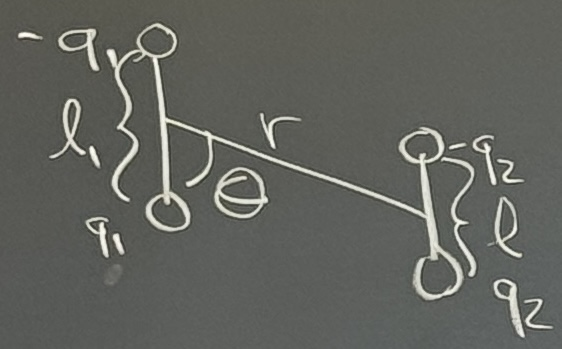
\includegraphics[width=0.2\linewidth]{intDplDpl.JPG}
        \caption{Schematic of a dipole-dipole interaction.}
        \label{fig:intDplDpl}
    \end{figure}
    \begin{itemize}
        \item Here, $\Delta E\propto 1/r^3$!
        \item If the dipoles align, this can stabilize the system, building up hierarchicial interactions that can even lead to self-assembly (e.g., in the case of polymers).
        \item Example: Solid-state NMR with \textbf{magic angle spinning}.
        \item See \textcite[168]{bib:Anslyn}.
    \end{itemize}
    \item \textbf{Magic angle spinning}: When you optimize the dipole-dipole interaction energy expression to have $E=0$ by setting $\theta=\ang{54.7}$ (aka, the "magic angle").
    \begin{figure}[h!]
        \centering
        \begin{subfigure}[b]{0.3\linewidth}
            \centering
            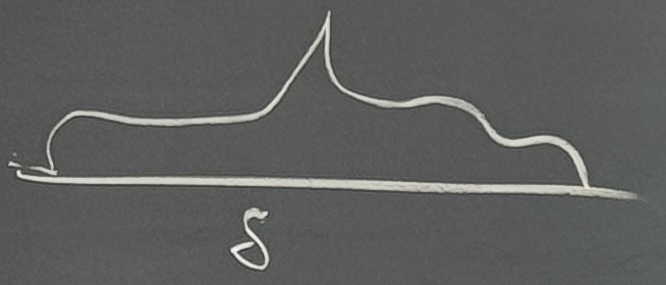
\includegraphics[width=0.8\linewidth]{magicAnglea.JPG}
            \caption{Without MAS.}
            \label{fig:magicAnglea}
        \end{subfigure}
        \begin{subfigure}[b]{0.3\linewidth}
            \centering
            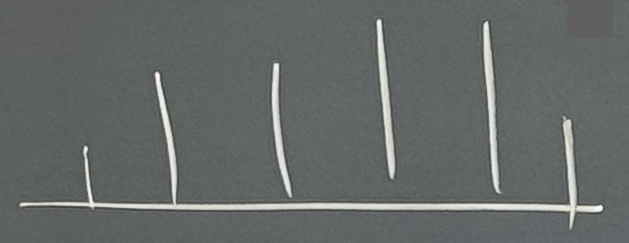
\includegraphics[width=0.8\linewidth]{magicAngleb.JPG}
            \caption{With MAS.}
            \label{fig:magicAngleb}
        \end{subfigure}
        \caption{Magic angle spinning.}
        \label{fig:magicAngle}
    \end{figure}
    \begin{itemize}
        \item Essentially, a "normal" solid-state NMR spectrum has a bunch of the anisotropy and broad linewidths.
        \item However, suppose we fix the sample in the magnetic field at \ang{54.7}. Then we spin the crap out of it ($\approx\SI{10000}{\revolutionsperminute}$). In this case, you get really fantastic tight lines from which you can read out the chemical shift tensor.
    \end{itemize}
    \item David: Why is there only one $\theta$ in Figure \ref{fig:intDplDpl}?
    \begin{itemize}
        \item Look at an intro physics or linear algebra textbook.
        \item There are more degrees of freedom that we can introduce, but this is all we need for right now. If the dipoles are not parallel or in the same plane, the equation gets more complicated but the critical $\Delta E\propto 1/r^3$ relation always remains true.
    \end{itemize}
    \item \textbf{Dipole-induced dipole} (interaction): An NCI in which one dipole induces a dipole in a \textbf{polarizable} molecule, and the two attract. \emph{Also known as} \textbf{Debye force}. \emph{Given by}
    \begin{equation*}
        E = \frac{\mu^2\alpha}{r^6}
    \end{equation*}
    \begin{itemize}
        \item Example: Taking a polar molecule (like water) and bringing it close to something polarizable like an arene, so that the two attract.
        \item See \textcite[187-88]{bib:Anslyn}.
    \end{itemize}
    \item \textbf{Polarizability}: The susceptibility of an atom or molecule's electron cloud to being pushed around or distorted. \emph{Denoted by} $\bm{\alpha}$.
    \begin{itemize}
        \item $\alpha$ is called the \textbf{polarizability tensor}.
        \item Indeed, polarizability can be quantified as a tensor (not a vector).
        \item See \textcite[24-25]{bib:Anslyn}.
    \end{itemize}
    \item \textbf{Disperson} (interaction): An NCI between the quantum-mechanically arising, correlated motions of electrons between molecules. \emph{Also known as} \textbf{London force}. \emph{Given by}
    \begin{equation*}
        E = \frac{\alpha_1\alpha_2}{r^6}
    \end{equation*}
    \emph{Schematic}
    \begin{figure}[h!]
        \centering
        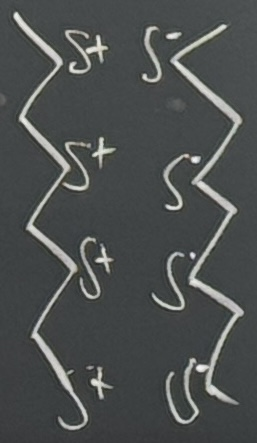
\includegraphics[width=0.1\linewidth]{intDis.JPG}
        \caption{Schematic of a dispersion interaction.}
        \label{fig:intDis}
    \end{figure}
    \begin{itemize}
        \item Any single electron induces a small correlation, but many electrons can induce some big correlations in bigger molecules.
        \begin{itemize}
            \item Longer molecules also maximize dispersion forces.
        \end{itemize}
        \item Governed by the Pauli exclusion principle: We can't fit more than two electrons into the same orbital, so electrons will still not "hop" between molecules.
    \end{itemize}
    \item Example of dispersion forces: Silylenes.
    \begin{figure}[H]
        \centering
        \begin{subfigure}[b]{0.2\linewidth}
            \centering
            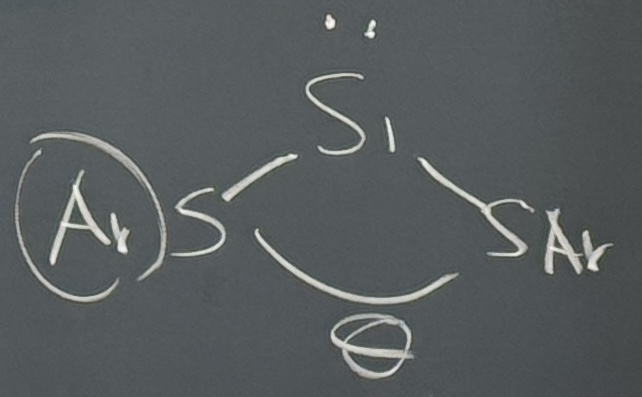
\includegraphics[width=0.8\linewidth]{silylenea.JPG}
            \caption{Silylene schematic.}
            \label{fig:silylenea}
        \end{subfigure}
        \begin{subfigure}[b]{0.4\linewidth}
            \centering
            \footnotesize
            \schemestart
                \chemfig{ArS-!{wave}}
                \arrow{0[\small $\equiv$][][-2mm]}
                \chemfig[atom sep=1.4em]{S-[4]*6(=(-*6(-(-[,0.8]R)=-(-[,0.8]R)=-(-[,0.8]R)=))-=-=(-*6(=(-[,0.8]R)-=(-[,0.8]R)-=(-[,0.8]R)-))-)}
            \schemestop
            \caption{Terphenyl thiolate ligands.}
            \label{fig:silyleneb}
        \end{subfigure}
        \caption{Dispersion forces bend silylenes.}
        \label{fig:silylene}
    \end{figure}
    \begin{itemize}
        \item Silylenes are the silicon analog of carbenes (Figure \ref{fig:silylenea}).
        \begin{itemize}
            \item We've already talked about carbene bending in this couse.
            \item Here's an additional note, though: There are both electronic \emph{and} steric reasons why a carbene would bend at a certain angle, since the electronic preference for some angle has to overcome the steric clash.
            \item The same is true of silylenes.
        \end{itemize}
        \item Consider a silylene with two terphenyl thiolate ligands (Figure \ref{fig:silyleneb}).
        \begin{itemize}
            \item Such ligands are a lot to look at, but they're really easy to make.
            \item When $\ce{R}=\ce{Me}$, $\theta\approx\ang{90.5}$.
            \begin{itemize}
                \item Note that this is a smaller angle than either singlet or triplet carbenes (see Figure \ref{fig:carbeneST}) because the heavier \textbf{congeners} of carbon tend to be more bent.
            \end{itemize}
            \item When $\ce{R}=\ce{{}^{\emph{i}}Pr}$, $\theta\approx\ang{84.8}$.
            \begin{itemize}
                \item Thus, when the terphenyl thiolate ligands are bulkier, the silylenes are \emph{more} bent!
                \item Steric repulsion is being overcome somehow.
            \end{itemize}
        \end{itemize}
        \item Why this counterintuitive result?
        \begin{itemize}
            \item Steric interactions are not necessarily repulsive! We've all been lied to.
            \item Why? Recall the \textbf{Lennard-Jones potential}.
            \begin{itemize}
                \item At large distances, two atoms have an energy as if they're not interacting at all.
                \item As you bring them together, you get a stabilizing interaction until the nuclei begin repulsing, giving you an equilibrium bond distance.
                \item Implication: Things must be \emph{very} close together to get steric repulsions; there are bonding interactions that occur at far greater systems.
                \item Steric properties of molecules are not always repulsive.
                \item This is a universe-level phenomenon that matter tends to condense.
                \item This is a profound insight that is animating a lot of method development in organic chemistry right now.
            \end{itemize}
        \end{itemize}
    \end{itemize}
    \item \textbf{Congeners}: Chemical substances related to each other by origin, structure, or function.
    \item \textbf{Lennard-Jones} (potential): A mathematical energy potential that fairly well approximates the energy of two binding atoms as they are brought closer together. \emph{Given by}
    \begin{equation*}
        E \propto \frac{A}{r^{12}}-\frac{B}{r^6}
    \end{equation*}
    \emph{Graph}
    \begin{figure}[h!]
        \centering
        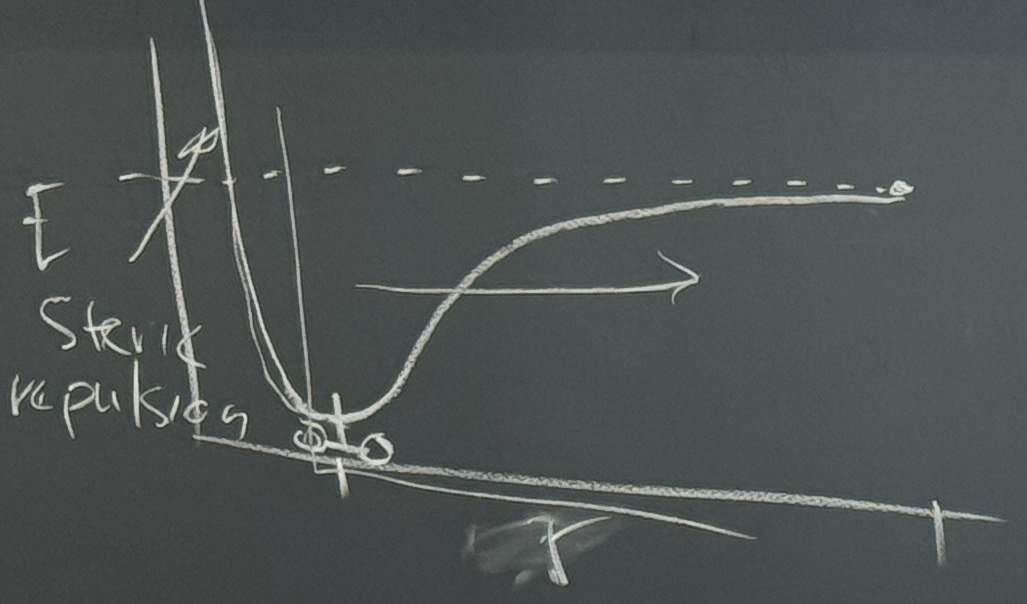
\includegraphics[width=0.3\linewidth]{intLJ.JPG}
        \caption{Lennard-Jones potential.}
        \label{fig:intLJ}
    \end{figure}
    \begin{itemize}
        \item Most Lennard-Jones potentials have the 12-6 form transcribed above.
    \end{itemize}
    \item This concludes our discussion of van der Waals interactions.
    \pagebreak
    \item \textbf{Quadrupole}: Something that has the shape/topology of a $d$-orbital.
    \item Examples of quadrupoles.
    \begin{figure}[h!]
        \centering
        \begin{subfigure}[b]{0.25\linewidth}
            \centering
            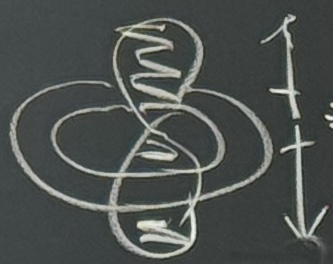
\includegraphics[width=0.7\linewidth]{quadrupoleExa.JPG}
            \caption{Quadrupolar orbital.}
            \label{fig:quadrupoleExa}
        \end{subfigure}
        \begin{subfigure}[b]{0.25\linewidth}
            \centering
            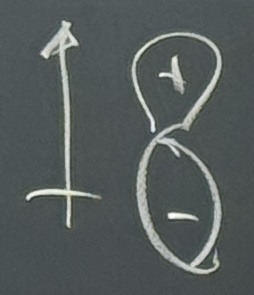
\includegraphics[width=0.45\linewidth]{quadrupoleExb.JPG}
            \caption{Dipolar orbital.}
            \label{fig:quadrupoleExb}
        \end{subfigure}
        \begin{subfigure}[b]{0.4\linewidth}
            \centering
            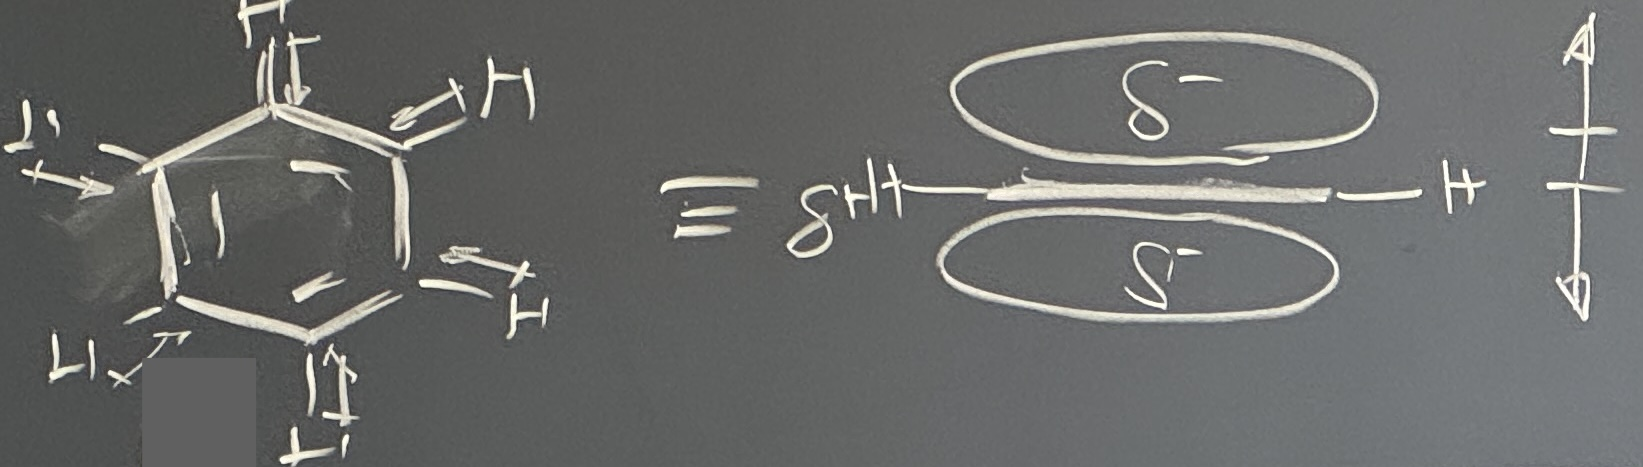
\includegraphics[width=0.95\linewidth]{quadrupoleExc.JPG}
            \caption{Quadrupolar molecule.}
            \label{fig:quadrupoleExc}
        \end{subfigure}
        \caption{Quadrupole examples.}
        \label{fig:quadrupoleEx}
    \end{figure}
    \begin{itemize}
        \item A $d_{z^2}$ orbital has two dipoles that cancel each other out (Figure \ref{fig:quadrupoleExa}).
        \begin{itemize}
            \item In contrast, dipoles are like $p$-orbitals (Figure \ref{fig:quadrupoleExb}).\footnote{Alex drew the dipole arrow in the inverse direction here by accident.}
            \item Note that orbitals aren't polar; these analogies are given to illustrate phasing properties.
        \end{itemize}
        \item You don't need a $d$-orbital to have a quadrupole, though --- they exist in organic chemistry, too!
        \item Example of quadrupolar molecules in organic chemistry: Benzene (Figure \ref{fig:quadrupoleExc}).
        \begin{itemize}
            \item All \ce{C-H} bonds have dipoles that cancel each other out.
            \item However, the net transfer of electron density increases the electron density in the $\pi$-cloud, even as it depletes the electron density at the hydrogens.
        \end{itemize}
        \item Example of quadrupolar molecules in organic chemistry: \ce{CO2}.
    \end{itemize}
    \item Just like we have charge-dipole interactions, we can have \textbf{charge-quadrupole} interactions.
    \item \textbf{Ion-quadrupole} (interaction): An NCI between a cation and the face of a quadrupole.
    \begin{itemize}
        \item Different atoms in the periodic table have different electronegativities, which we know thanks to Linus Pauling's building on Dmitri Mendeleev's foundation.
        \item These are most commonly encountered when we have an arene and we bring in an ion on top.
        \begin{itemize}
            \item Leads to a net-stabilizing interaction between the ion and the charged molecule.
        \end{itemize}
        \item See \textcite[181-83]{bib:Anslyn}.
    \end{itemize}
    \item Example: \ce{K+} and benzene.
    \begin{figure}[h!]
        \centering
        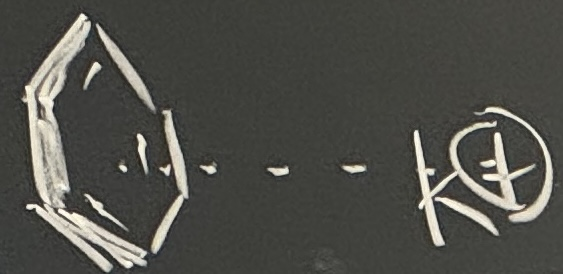
\includegraphics[width=0.2\linewidth]{Kbenz.JPG}
        \caption{Ion-quadrupole interaction of \ce{K+} and benzene.}
        \label{fig:Kbenz}
    \end{figure}
    \begin{itemize}
        \item These two species' gas phase binding enthalpy is $\Delta H=-\kcal{19}$.
        \item For comparison, the gas phase binding enthalpy of \ce{K+} and \ce{H2O} is $\Delta H=-\kcal{18}$.
        \begin{itemize}
            \item This shows that ion-dipole and ion-quadrupole interactions are about similarly intense, even though benzene doesn't really have charged regions.
            \item This is surprising, in Alex's opinion.
        \end{itemize}
        \item Reference: \textcite{bib:Kbenz}.
    \end{itemize}
    \pagebreak
    \item Example: Ions and benzene.
    \begin{table}[h!]
        \centering
        \small
        \renewcommand{\arraystretch}{1.2}
        \begin{tabular}{cc}
            \textbf{\ce{M+}} & $\bm{-\Delta H}$\\
            \hline
            \ce{Li+}   & $38.3$\\
            \ce{Na+}   & $28.0$\\
            \ce{K+}    & $19.2$\\
            \ce{NH4+}  & $19.3$\\
            \ce{NMe4+} & $9.4$ \\
        \end{tabular}
        \caption{Ion-quadrupole interactions with benzene.}
        \label{tab:intQua}
    \end{table}
    \begin{itemize}
        \item Ion-quadrupole interactions are subject to a size dependence.
        \item Specifically, harder ions bind better to quadrupoles, and softer ones binds worse.
        \item This is consistent with the inverse distance dependence in all of our interaction equations.\footnote{Note: HSAB (as a polarizability- and dispersion-directed phenomenon) does indeed favor the binding of "soft" benzene to "soft" ions, but the fact that we see this relationship here implies that electrostatics (i.e., classical ion-quadrupole attractions) are \emph{more} active in determing benzene's affinity for cations \parencite[163-64]{bib:intQuaBio}.}
        \item See \textcite{bib:intQuaBio}, specifically the section entitled "The Fundamental Interaction: Gas-Phase Studies" and refs. 2-7 cited therein.
    \end{itemize}
    \item Example: The effect of arene substituents on ion-quadrupole interactions.
    \begin{itemize}
        \item Look it up if we're so inclined!!
        \item Alex goes deep into this topic many years, "but this year, I'm like f it."
        \item Reference: \textcite{bib:ionQuaSubs}.
        \begin{itemize}
            \item By Dennis Dougherty, of \textcite{bib:Anslyn}!
        \end{itemize}
    \end{itemize}
    \item Example: Cation-$\pi$ interactions in biology.
    \begin{itemize}
        \item Proteins stabilize charged species within them, even when solvated in a high dielectric (\ce{H2O}) at physiological $\pH$ ($\pH\approx 7$). How do they do this?
        \begin{itemize}
            \item Water is great at solvating charged species, so to incorporate charged species, proteins have to pay a desolvation penalty.
            \item Proteins definitely don't work by allowing water inside them: In fact, enzymes and proteins adopt a tertiary structure that often excludes water into the bulk.
            \item Thus, the solution is that proteins use ion-quadrupole interactions (with aromatic residues).
        \end{itemize}
        \item Takeaway: Nonpolar, hydrophobic arenes can stabilize cations even in aqueous media.
        \item Example: Would benzene or a carboxylate anion stabilize the trimethylammonium cation more?
        \begin{itemize}
            \item Gas phase: The binding of trimethylammonium to benzene ($\Delta H=-\kcal{19}$) is far more stabilizing than its binding to acetate ($\Delta H>\kcal{100}$).
            \item In water: There is so much dielectric stabilization that binding to benzene is weaker ($\Delta H=-\kcal{5.5}$), and binding to acetate doesn't do that much at all ($\Delta H=-\kcal{2.2}$).
        \end{itemize}
        \item Corollary: Proteins can take carboxylic acids and modulate their $\pKa$ over multiple log-units via enclosure in a hydrophobic environment.
        \item Aside: This is a case of a biological phenomenon being explained by physical chemistry.
        \begin{itemize}
            \item If you believe that biology lends greater insight into the physical world, good for you!
            \item Alex, personally, would rather just look at physical systems though.
        \end{itemize}
        \item Reference: \textcite{bib:intQuaBio}.
        \begin{itemize}
            \item By Dennis Dougherty again!
        \end{itemize}
    \end{itemize}
    \item \textbf{Apparent} (interaction): An NCI that is frequently alluded to in the literature, real, and yet has no fundamental physical basis.
    \begin{itemize}
        \item This is Alex's term; we won't hear about "apparent" interactions anywhere else.
        \item Several subsets.
        \begin{enumerate}[label={\Roman*.)}]
            \item \textbf{$\bm{\pi}$-$\bm{\pi}$ interactions}.
            \item \textbf{Hydrogen bonds}.
        \end{enumerate}
    \end{itemize}
    \item \textbf{$\bm{\pi}$-$\bm{\pi}$} (interaction): An NCI between two (typically aromatic) $\pi$-systems.
    \begin{itemize}
        \item The physical basis for such interactions is probably very complex.
        \item See \textcite[184]{bib:Anslyn}.
    \end{itemize}
    \item There are three main types of $\pi$-$\pi$ interaction geometries.
    \begin{figure}[h!]
        \centering
        \begin{subfigure}[b]{0.25\linewidth}
            \centering
            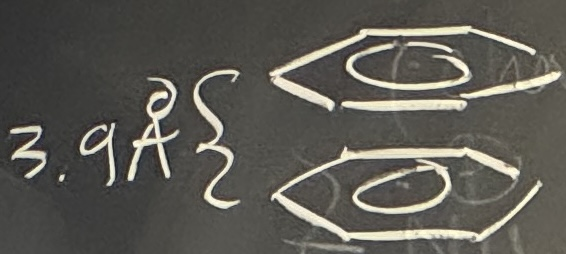
\includegraphics[width=0.8\linewidth]{piPiGeoa.JPG}
            \caption{Parallel stack.}
            \label{fig:piPiGeoa}
        \end{subfigure}
        \begin{subfigure}[b]{0.25\linewidth}
            \centering
            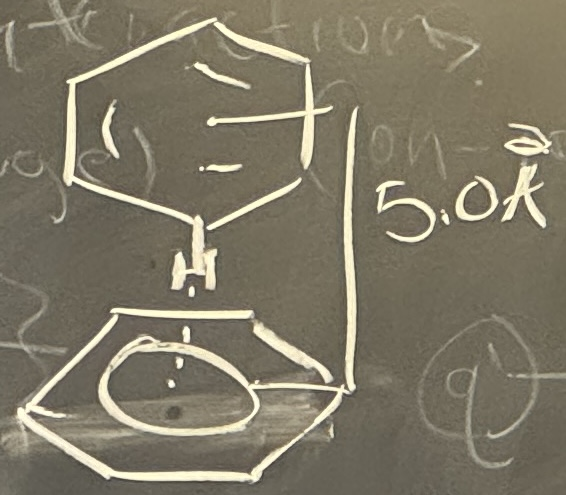
\includegraphics[width=0.65\linewidth]{piPiGeob.JPG}
            \caption{T-shaped.}
            \label{fig:piPiGeob}
        \end{subfigure}
        \begin{subfigure}[b]{0.25\linewidth}
            \centering
            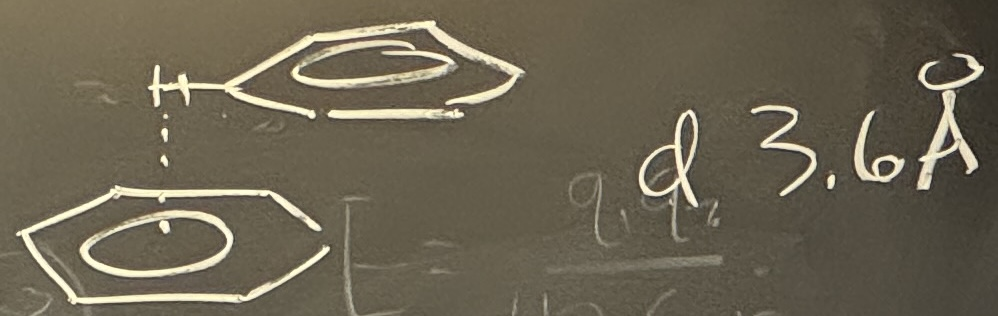
\includegraphics[width=0.98\linewidth]{piPiGeoc.JPG}
            \caption{Slipped stack.}
            \label{fig:piPiGeoc}
        \end{subfigure}
        \caption{$\pi$-$\pi$ interaction geometries.}
        \label{fig:piPiGeo}
    \end{figure}
    \begin{enumerate}
        \item The \textbf{parallel stack} of two centroids.
        \item The \textbf{T-shaped geometry}.
        \item The \textbf{slipped stack geometry}.
    \end{enumerate}
    \item \textbf{Parallel stack} (geometry): A $\pi$-$\pi$ interaction geometry in which the two centroids stack their $\pi$-systems on top of each other.
    \begin{itemize}
        \item The equilibrium distance is about \SI{3.9}{\angstrom}.
        \item Important for electronic transport through adjacent $\pi$-systems, but not relevant to us today.
        \item Energy: $\Delta H=-\kcal{1.7}$.
    \end{itemize}
    \item \textbf{T-shaped} (geometry): A $\pi$-$\pi$ interaction geometry in which a region of negative electrostatic potential (the face of one ring) is in contact with a region of positive electrostatic potential (the edge of the other). \emph{Also known as} \textbf{edge-to-face}.
    \begin{itemize}
        \item The equilibrium distance is about \SI{5.0}{\angstrom}.
        \item Energy: $\Delta H=-\kcal{2.6}$.
        \begin{itemize}
            \item This is more stable than the $\pi$-stack!
        \end{itemize}
    \end{itemize}
    \item \textbf{Slipped stack} (geometry): A $\pi$-$\pi$ interaction geometry consisting of coplanar $\pi$-systems with a dislocation between the centroids. \emph{Also known as} \textbf{displaced}.
    \begin{itemize}
        \item The equilibrium distance is about \SI{3.6}{\angstrom}.
        \item Energy: $\Delta H=-\kcal{2.6}$.
        \begin{itemize}
            \item Thus, this geometry is still more stable than the conventional parallel stack.
        \end{itemize}
    \end{itemize}
    \item Implication: There's nothing intrinsic about arenes that makes them want to $\pi$-$\pi$ stack, and this phenomenon will be generalized to other types of species.
    \item There are two main models through which to view the phenomenon of $\pi$-$\pi$ interactions.
    \begin{enumerate}
        \item The \textbf{Wheeler-Houk model}.\footnote{"HOWK"}
        \item The \textbf{Grimme dispersion model}.\footnote{"shteh-FAHN GRIM-uh," a professor at the University of Bonne.}
        \item As a possible third, Brent Iverson (UT-Austin) has many beautiful papers on $\pi$-$\pi$ stacking.
        \begin{itemize}
            \item The papers are a bit pedantic, but "I'm [Alex is] a pedant."
        \end{itemize}
    \end{enumerate}
    \item \textbf{Wheeler-Houk} (model): A model of $\pi$-$\pi$ stacking predicated on direct interactions.
    \begin{itemize}
        \item Wheeler and Houk found (computationally and experimentally) that it's not the $\pi$-faces that interact, but the substituents on the arene that have a quadrupolar interaction with the other arene below.
        \item Their model works for substituted arenes.
        \item Reference: \textcite{bib:WheelerHouk}.
    \end{itemize}
    \item \textbf{Grimme dispersion} (model): A model of $\pi$-$\pi$ stacking which posits that more extended $\pi$-sytems facilitate and maximize disperson.
    \begin{itemize}
        \item This model is more descriptive as we get to larger $\pi$-systems.
    \end{itemize}
    \item This concludes our discussion of $\pi$-$\pi$ interactions; we now move onto hydrogen bonding.
    \item \textbf{Hydrogen bond}: An NCI between a donor of the form \ce{A-H} and an acceptor of the form \ce{B}. \emph{Schematic}
    \begin{figure}[h!]
        \centering
        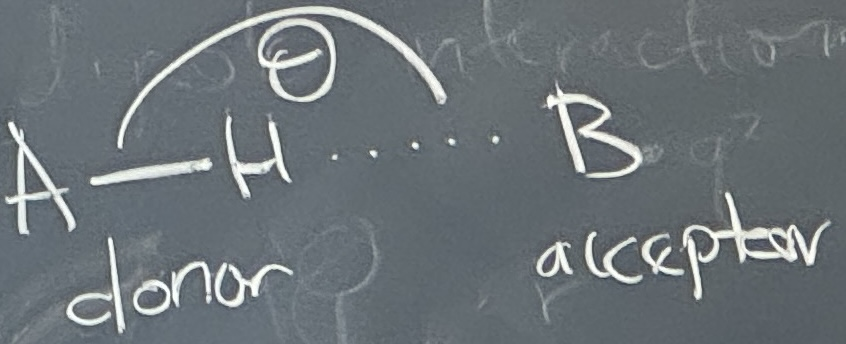
\includegraphics[width=0.25\linewidth]{intHbond.JPG}
        \caption{Schematic of a hydrogen bond.}
        \label{fig:intHbond}
    \end{figure}
    \begin{itemize}
        \item This is a really ill-defined suite of physical phenomena that --- all the same --- we humans can classify really well.
        \begin{itemize}
            \item There is (at least) an electrostatic component, an ion-dipole moment, some covalency, etc.
        \end{itemize}
        \item Review (the sacred text of hydrogen bonds): \textcite{bib:Hbond}.
        \item There is a continuum of hydrogen bonds --- from strong to moderate to weak --- that is characterized by the distance between the \ce{H}-bond donor and acceptor as well as the angle, resulting in an energy of stabilization.
        \begin{itemize}
            \item Strong: \SIrange{1.2}{1.5}{\angstrom} and $\theta=\angrange{175}{180}$, $\Delta E=\kcalr{14}{40}$.
            \begin{itemize}
                \item Large degree of covalency.
            \end{itemize}
            \item Moderate: \SIrange{1.5}{2.2}{\angstrom} and $\theta=\angrange{130}{180}$, $\Delta E=\kcalr{4}{15}$.
            \begin{itemize}
                \item More electrostatic in nature.
            \end{itemize}
            \item Weak: \SIrange{2.3}{3.2}{\angstrom} and $\theta=\angrange{90}{150}$, $\Delta E<\kcal{4}$.
            \begin{itemize}
                \item Even \kcal{4} can upend selectivity.
                \item Thus, even these are important!
            \end{itemize}
        \end{itemize}
    \end{itemize}
\end{itemize}




\end{document}